\documentclass[a4paper,12pt]{report}

% Packages
\usepackage[dutch]{babel}           
\usepackage[latin1]{inputenc}       	% speciale karakters
\usepackage{graphicx} 					% figuren

\usepackage{enumitem}
\usepackage{longtable}
\usepackage{array}
\usepackage[hyphens]{url}
\usepackage{pdfpages}
\usepackage{amssymb}
\usepackage{amsmath}
\usepackage{graphicx}
\usepackage[font=small,format=plain,labelfont=bf,up,textfont=it,up]{caption}
\usepackage{float}
\usepackage[bottom]{footmisc}
\usepackage[T1]{fontenc}
\usepackage{lastpage}
\usepackage{fancyhdr}
\usepackage{caption}
\usepackage{subcaption}
\usepackage{varioref}
\usepackage{hyperref}

% Optional settings

\setlength{\hoffset}{-1cm}         
\addtolength{\textwidth}{2cm}
\setlength{\voffset}{-1cm}
\addtolength{\textheight}{2cm}

\setcounter{tocdepth}{1}
\setcounter{secnumdepth}{3}
\def\thesection{\arabic{section}}

\pagestyle{fancy}
\lhead{Dieter Decaestecker, Tom Naessens}
\rhead{Verslag project Hoog-performant rekenen}

\newcommand{\niceref}[1]{\autoref{#1} on \autopageref{#1}}

\parindent 0pt
\begin{document}
\begin{titlepage}
\fontsize{12pt}{14pt}\selectfont
\begin{center}
% Logo of the university Gent
\includegraphics[height=3cm]{images/ugent.pdf}

\vspace{1cm}

\fontsize{14pt}{17pt}\selectfont
% De Faculty:
\textsc{Faculteit Ingenieurswetenschappen}
\fontsize{12pt}{14pt}\selectfont
\vspace{0.3cm}

\vspace{1.2cm}

% Academy year
Academiejaar 2014-2015

\vspace{3cm}

\fontsize{17.28pt}{21pt}\selectfont

% Title of the report.
{\textsc{Project Vage Databanken}}

\fontseries{m}
\fontsize{12pt}{14pt}\selectfont

\vspace{4cm}

% Names of the author.
   Tom Naessens\\
   Nick Van Haver\\

\end{center}
\thispagestyle{empty}
\end{titlepage}



\section{Probleemstelling}

Ons doel is om het volgend stelsel op te lossen op een computationeel snelle manier:

\begin{equation*}
\overbrace{\begin{bmatrix} X^TX & X^TZ \\ Z^TX & Z^TZ+\frac{\sigma_e^2}{\sigma_s^2}I \end{bmatrix}}^{\text{$A$, gegeven}} \underbrace{ \left[ \begin{array}{c} b \\ u \end{array} \right]}_{\text{$x$, gevraagd}} =  \overbrace{\left[ \begin{array}{c} X^Ty \\ Z^Ty \end{array} \right]}^{\text{$B$, gegeven}} \\
\end{equation*}

De aangeduide benamingen zullen we ook gebruiken doorheen de rest van dit verslag. Zoals aangegeven is de data om de matrix $A$ en de vector $y$ op te stellen gegeven.

Concreet zijn de volgende problemen op te lossen:
\begin{enumerate}
\item Het opstellen van de 2 matrixes op basis van de gegeven data.
\item Het oplossen van de vergelijking a.d.h.v deze 2 matrixes.
\item Het berekenen van $\hat{y}$ en de determinatieco\"effici\"ent.
\end{enumerate}

Willen we dit probleem oplossen voor de gegeven inputdata hebben we een aanzienlijk hoeveelheid geheugen nodig om de matrixes in het geheugen te houden. Daarnaast zijn er ook een aanzienlijk hoge hoeveelheid operaties nodig om de matrix-matrix vermenigvuldigingen op te lossen (voornamelijk dankzij de bewerkingen waar de $Z$ matrix deel van uitmaakt).
Een HPR-oplossing is voor dit probleem dan ook uiterst geschikt: matrix-matrix vermenigvuldigingen zijn sterk parallelliseerbaar en voor dit soort operaties worden ook standaard implementaties aangeboden door HPR softwarebibliotheken. In het bijzonder door de bibliotheek die wij zullen gebruiken; ScaLAPACK. 

\section{High-level overzicht van de oplossing}
We hebben voornamelijk gebruik gemaakt van de voorgestelde parallelle oplossing (de gebruikte ScaLAPACK functies zijn telkens tussen haakjes vermeld):

\begin{enumerate}
	\item Initialisatie van MPI en van het procesraster (dit laatste aan de hand van de functies \texttt{sl\_init\_ en blacs\_gridinfo\_}).
	\item De data wordt ingelezen en verspreid vanaf het rootproces:
	\begin{enumerate}
		\item De bestanden $X$, $Y$ en $Z$ worden beschreven aan de hand van \texttt{descinit\_}.
		\item Het rootproces leest de data in $X$ en $Y$ en verspreid deze blokcylisch onder de processen (aan de hand van \texttt{dgesd2d\_} en \texttt{dgerv2d\_}).
		\item Het rootproces leest enkele lijnen van de het $Z$ bestand in, berekent de matrixlijn van $Z$ en verspreid deze lijn blokcylisch naar de verschillende processen. Dit gaat door tot $Z$ volledig ingelezen en verspreid is.
	\end{enumerate}
	\item $A$ wordt opgesteld en berekend:
	\begin{enumerate}
		\item De matrix $A$ wordt beschreven aan de hand van \texttt{descinit\_}.
		\item $A$ wordt gevuld (aan de hand van \texttt{pdlaset\_}) met de foutco\"effici\"ent op de diagonaal.
		\item De deelmatrices van $A$: $X^TX$, $X^TZ$, $Z^TX$ en $Z^TZ$ worden berekend (via \texttt{pdgemm\_}) en worden op hun correcte plaats in $A$ geplaatst door een offset mee te geven aan de \texttt{pdgemm\_} oproep.
	\end{enumerate}
	\item $B$ wordt opgesteld en berekend:
		\begin{enumerate}
			\item De vector $B$ wordt beschreven (aan de hand van \texttt{descinit\_}).
			\item De deelvectoren van $B$: $X^TY$ en $Z^TY$ worden berekend via \texttt{pdgemv\_} en worden op hun plaats in $B$ geplaatst door een offset mee te geven aan de \texttt{pdgemv\_} oproep.
		\end{enumerate}
	\item Het stelsel wordt opgelost (aan de hand van \texttt{pdgesv\_}). Hierbij wordt $A$ overschreven door zijn LU-factorisatie en $B$ door de oplossing van het stelsel.
	\item De evaluatieresultaten worden berekend en verzameld op het rootproces:
		\begin{enumerate}
			\item De oplossing van het stelsel terug verzameld (aan de hand van \texttt{dgesd2d\_} en \texttt{dgerv2d\_}).
			\item $\hat{y}$ wordt beschreven (aan de hand van \texttt{descinit\_}) en berekend door (aan de hand van \texttt{pdgemv\_}) $X*b$ en $Z*u$ op te tellen bij deze lege vector.
			\item $\hat{y}$ wordt terug verzameld op het rootproces.
		\end{enumerate}
\end{enumerate}

Een single-core/node implementatie is quasi onmogelijk vanwege de redenen beschreven in deel 1, in deel 3.3 gaan we hier dieper op in.

De grootste bottleneck is sowieso het inlezen van de matrices uit de opgegeven bestanden. Dit is een IO-gebonden proces dat niet of zeer moeilijk te paralleliseren is. Momenteel leest het rootproces alle bestanden in en verdeelt deze onder de overige processen. Mocht dit geperalleliseerd worden zou dit veel versneld kunnen worden. Voor bijvoorbeeld 96 processen neemt het uitvoeren van de vermenigvuldigingen zelf 208 seconden in beslag. Het inlezen echter 4305 seconden. Dit is dus een gigantische bottleneck. Meer over de resultaten bespreken we in deel \ref{resultaten} op pagina \pageref{resultaten}.

Een ander probleem waar we tegen aan zijn gelopen is dat niet enkel het berekenen van $Z^TZ$ te zwaar is voor \'e\'en proces, maar zelfs het inlezen van de data voor en omzetten naar $Z$ is te data-intensief. Daarom hebben we het inlezen en het verdelen van de data gecombineerd zodat de data iteratief in kleine stukken wordt ingelezen en verspreid. Omdat $X$ en $Y$ een stuk kleiner zijn was het wel mogelijk om deze data eerst volledig in te lezen en dan te verspreiden. Voor grotere datasets zal een soortgelijke oplossing zoals $Z$ ook nodig zijn voor $X$ en $Y$.

\section{Kwaliteitsmetrieken}
\subsection{Aantonen juistheid}
We kunnen de juistheid aantonen aan de hand van drie metrieken:

Ten eerste zouden de waarden van de $b$ vector, zoals vermeld in de opgave, in de buurt moeten liggen van [100, 1]. De bekomen waarden voor $b$ van het kleine model zijn [110.869, 1.04896]. Voor het grote model bekomen we [99.4539, 1.00051].

Daarnaast zou de correlatie van $Y$ en $\hat{Y}$ overeen moeten komen. Dit kunnen we berekenen aan de hand van de determinatieco\"effici\"ent $R^2$. Voor het kleine model is $R^2$ gelijk aan 0.8722 en voor het grote model 0.9132.

Als laatste zou de bekomen $u$ vector een normaaldistributie moeten volgen. In figuur \ref{Udistr} op pagina \pageref{Udistr} staat een genormaliseerd histogram van de waarden in $u$ met de normaaldistributie in het rood. 

Alle metrieken liggen zeer dicht bij de verwachte en benodigde waarden. We kunnen er dus van uit gaan dat onze oplossing correct is voor zowel het kleine als het grote model.

\begin{figure}
    \centering
    \includegraphics[width=0.5\textwidth]{includes/u-big}
    \caption{Genormaliseerde distributie van $u$ tegenover de normaaldistributie (in het rood weergegeven)}
    \label{Udistr}
\end{figure}

\subsection{Bespreking resultaten}
\label{resultaten}
We hebben als visuele voorstelling van de resultaten voor beide modellen de $Y$ vs $\hat{Y}$ verhouding geplot, zie hiervoor figuur \ref{YvsYHatGraphs} op pagina \pageref{YvsYHatGraphs}. Zoals in voorgaand puntje hebben we ook de determinatieco\"effici\"ent berekend. De lineaire regressielijn is in het rood als overlay toegevoegd aan de plots.
\begin{figure}
        \centering
        \begin{subfigure}[b]{0.45\textwidth}
                \includegraphics[width=\textwidth]{includes/Y-YHat-small}
                \caption{Klein model}
        \end{subfigure}
        \begin{subfigure}[b]{0.45\textwidth}
                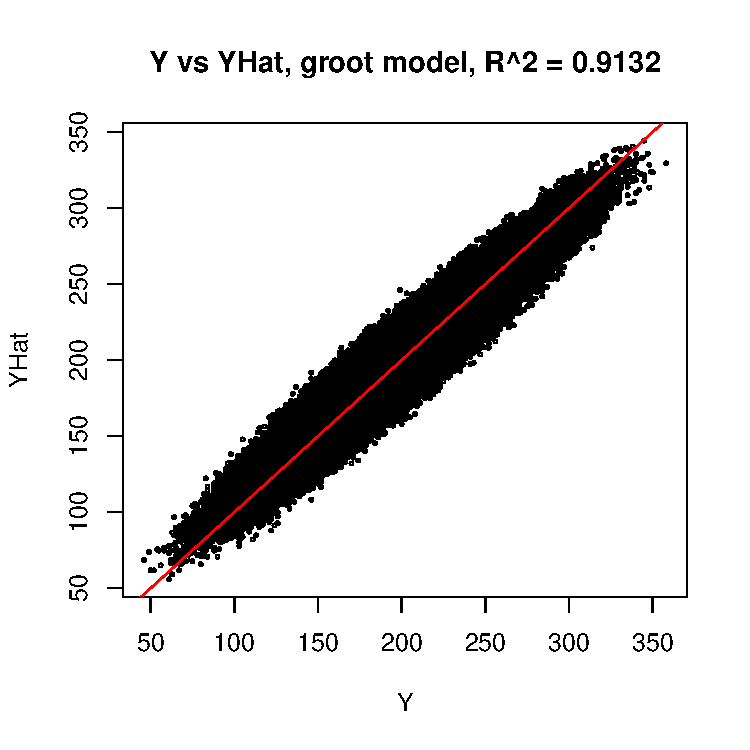
\includegraphics[width=\textwidth]{includes/Y-YHat-big.png}
                \caption{Groot model}
        \end{subfigure}
        \caption{$Y$ versus $\hat{Y}$}
        \label{YvsYHatGraphs}
\end{figure}

We zien duidelijk dat voor beide modellen de waarden zich langs de diagonaal bevinden. Dit duidt op een goeie fitting van het model.

\subsection{Bespreking HPC-aspect}
In figuur \ref{speed} op pagina \pageref{speed} is een grafiek te vinden van het aantal processen ten opzichte van de uitvoeringstijd. We brengen twee opzichten in rekening: enerzijds de volledige uitvoeringstijd van begin tot einde (inclusief het inlezen van de data) en anderzijds de tijd nodig om het stelsel zelf op te lossen (exclusief het inlezen van data). We zien duidelijk dat het inlezen van de data de grootste overhead vormt. Bij 96 processen bedraagt dit $\pm95$\% van de volledige tijd. Vandaar ook dat er tussen de verschillende volledige uitvoeringstijden weinig verschil te zien is. 

Als we naar de groene curve kijken, die enkel de berekeningen voorstelt, zien we wel een duidelijke daling van uitvoeringstijd bij het toenemen van het aantal processen. In tabel \ref{speeduptabel} of pagina \pageref{speed} is een overzicht te vinden van de speedup tegenover het miminum aantal benodigde processen, namelijk 32. Met een lager aantal processen dan 32 kon het probleem niet worden opgelost op de Delcatty cluster wegens geheugenlimieten.

We zien duidelijk dat de uitvoeringstijd van de bewerkingen halveert als het aantal processen verdubbeld. Hieruit kunnen we besluiten dat dit probleem goed schaalt ten opzichte van het aantal gebruikte processen en ook zeer goed te paralleliseren is.

\begin{table}
\centering
	\caption{Speedup voor de verschillende uitvoeringstijden per proces, met als basis de uitvoeringstijd op 32 processen.}
	\begin{tabular}{c|c|c}
	\#Processen & Uitvoeringstijd (s) & Speedup \\ 
	\hline \hline 32 & 550 & 100\% \\ 
	\hline 48 & 382 & 143\% \\ 
	\hline 64 & 270 & 204\% \\ 
	\hline 96 & 208 & 264\% \\  
	\end{tabular}
	\label{speeduptabel}
\end{table}

\begin{figure}
    \centering
    \includegraphics[width=0.5\textwidth]{includes/speed}
    \caption{Uitvoeringstijden tegenover gebruikt aantal processen}
    \label{speed}
\end{figure}

Een single-core/node oplossing is niet mogelijk voor dit probleem op de huidige Delcatty infrastructuur. De matrix die we dienen te vermenigvuldigen bestaat uit 1M rijen van 10.000 doubles. Dit resulteert in een geheugengebruik van ($1.000.000*10.000*8B=$) 80GB. Een node op de Delcatty cluster heeft een fysiek geheugen van 62.9GB, deze matrix past dus niet in het geheugen. Mocht de dataset kleiner zijn en wel binnen het geheugen passen van 1 node, is dit wel oplosbaar, ook al zal dit dan zeer lang duren.
Een single-core/node oplossing zou enkel mogelijk zijn moest de infrastructuur voldoende geheugen hebben en als de gebruiker veel geduld heeft.

\subsection{Conclusie}
We kunnen kort concluderen dat de berekeningen nodig om dit probleem op te lossen zeer goed te paralleliseren zijn. Het inlezen van de data is de grootste bottleneck. Mocht dit ook geparalleliseerd worden zou de volledige uitvoeringstijd sterk afnemen.
\end{document}
  